\documentclass[a4paper, 12pt]{report}

%%%%%%%%%%%%
% Packages %
%%%%%%%%%%%%

\usepackage[english]{babel}
\usepackage[noheader]{packages/sleek}
\usepackage{packages/sleek-title}
\usepackage{packages/sleek-theorems}
\usepackage{packages/sleek-listings}

% Custom colors
\usepackage{color}
\definecolor{deepblue}{rgb}{0,0,0.5}
\definecolor{deepred}{rgb}{0.6,0,0}
\definecolor{deepgreen}{rgb}{0,0.5,0}

%Per scrivere codice
\usepackage{listings}

\usepackage{pythonhighlight}

% Per figure nel testo
\usepackage{wrapfig}

% Per aggiungere ``Page 1 of 100''
\usepackage{lastpage}

\usepackage{mathtools}


\lstset{
	frame = single,
	numbers=left,                   % where to put the line-numbers
	numberstyle=\footnotesize,  % the style that is used for the line-numbers
	stepnumber=1,                   % the step between two line-numbers. If it is 1, each line
	numbersep=8pt                  % how far the line-numbers are from the code  
}

%\cfoot{\thepage\ of \label{LastPage}}
\cfoot{Page \thepage \hspace{1pt} of \pageref{LastPage}}

%%%%%%%%%%%%%%
% Title-page %
%%%%%%%%%%%%%%

\logo{./resources/img/logo.png}
\institute{Ca' Foscari University}
\faculty{Faculty of Computer Science}
%\department{Department of Anything but Psychology}
\title{Cryptography}
\subtitle{Afternotes}
\author{\textit{Author}\\Francesco \textsc{Vivian}}
%\supervisor{Linus \textsc{Torvalds}}
%\context{Well, I was bored...}
\date{A.Y. 2020-2021}

%%%%%%%%%%%%%%%%
% Bibliography %
%%%%%%%%%%%%%%%%

\addbibresource{./resources/bib/references.bib}

%%%%%%%%%%
% Others %
%%%%%%%%%%

\lstdefinestyle{latex}{
    language=TeX,
    style=default,
    %%%%%
    commentstyle=\ForestGreen,
    keywordstyle=\TrueBlue,
    stringstyle=\VeronicaPurple,
    emphstyle=\TrueBlue,
    %%%%%
    emph={LaTeX, usepackage, textit, textbf, textsc}
}

\FrameTBStyle{latex}

\def\tbs{\textbackslash}

%%%%%%%%%%%%
% Document %
%%%%%%%%%%%%

\newtheorem{definition}{\textbf{Definition}}
\newtheorem{property}{\textbf{Property}}
\newtheorem{example}{\textbf{Example}}
\newtheorem{exercise}{\textbf{Exercise}}
\newtheorem{theorem}{\textbf{Theorem}}

\begin{document}
    \maketitle
    %\romantableofcontents
\chapter*{Lecture 1}
\begin{definition}
	Security: it generically refers to the possibility of "protecting" information, which is either stored in a computer system or transmitted on a network.
\end{definition}
Whatever will be shown works in both situations.\\
To decide whether a computer system is "secure", you must first decide what secure means to you, then identify the threats you care about. Some threats are: cyberterrorism, denial of service, modified databases, virus, identity theft, stolen customer data, equipment theft, espionage.

\vspace{5mm}
There are different aspects to protect through security properties:
\begin{property}
	Authenticity: an entity should be correctly identified.
\end{property}
\begin{example}
	Some examples of authenticity:
	\begin{itemize}
		\item login process for authenticating a user (User Identification)
		\item a digital signature allows for authenticating the entity originating a message (Message Authentication)
	\end{itemize}
\end{example}
\vspace{5mm}
\begin{property}
	Confidentiality (secrecy): information should only be accessed (read) by authorized entities.
	\begin{itemize}
		\item Confidential information is not disclosed to unauthorized individuals (Data confidentiality)
		\item Individuals control what information related to them may be collected and stored and by whom that information may be disclosed (Privacy)
	\end{itemize}
\end{property}
\begin{example}
	Some examples of confidentiality:
	\begin{itemize}
		\item the person that accesses a database should be authorized to access the data
		\item personal privacy, my private data should be protected while browsing the web
	\end{itemize}
\end{example}
The "access control" for confidentiality:
\begin{itemize}
	\item use the "need to know" basis for data access. How do we know who needs what data? (Approach: access control specifies who can access what). How do we know a user is the person she claims to be? We need her identity and we need to verify this identity (Approach: identification and authentication).
	\item Analogously, the "need to access/use" is the basis for access to physical assets (access to a computer room, use of a desktop)
\end{itemize}
Confidentiality is difficult to ensure and easy to assess in terms of success: it is binary in nature (Yes/No).
\vspace{5mm}
\begin{property}
	Integrity: information should only be modified by authorized entities.
	\begin{itemize}
		\item information and programs are changed only in a specified and authorized manner (Data integrity)
		\item a system performs its intended function, free from unauthorized manipulation (System integrity)
	\end{itemize}
\end{property}
\begin{example}
	We should not alter bank accounts and IoT device firmware.
\end{example}
If we don't have integrity, we also don't have confidentiality (with integrity I want only authorized users to be able to modify information, with confidentiality I want only authorized users to be able to see information, modifying includes seeing).
Integrity is more difficult to to measure than confidentiality, it is non binary (it has degrees of integrity) and it is content-dependent (it means different things in different context)
\begin{example}
	A quotation from a politician, we can preserve the quotation (data integrity) but mis-attribute (origin integrity), like \textit{Y said that} instead of \textit{X said that}. 
\end{example}
\vspace{5mm}
\begin{property}
	Availability: information should be available/usable fastly by authorized users.
\end{property}
\begin{example}
	It is important to guarantee reliability and safety. Apart from attacks, availability might be loss in case of faults (we need to use fault-tolerant techniques). We need availability in case of a remote surgery for example (good QoS).
\end{example}
We can say that an asset (a resource) is available if:
\begin{itemize}
	\item it provides a timely request response
	\item it provides fair allocation of resources (no starvation)
	\item it is fault tolerant (no total breakdown)
	\item it is easy to use in the intended way
	\item it provides controlled concurrency (concurrency control, deadlock control, ..)
\end{itemize}
\vspace{5mm}
\begin{property}
	Non-repudiation: an entity should not be able to deny an event. 
\end{property}
\begin{example}
	Having sent/received a message. This property is crucial for e-commerce, where "contracts" should not be denied by parties.
\end{example}
\vspace{5mm}
Other properties that are not addressed in detail are: fairness of contract signing, privacy, anonimity and unlinkability, accountability, ..
\subsubsection{Typical attacks}
We will now see some typical attacks. We assume that information is flowing from a source to a destination (e.g.: reading data is a flow from the data container to a user, writing is a flow from a user to the file system).\\

\begin{wrapfigure}[9]{l}{0.4\textwidth}
	%\centering
	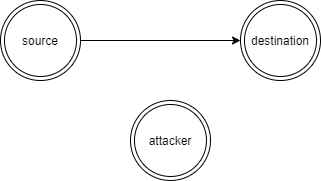
\includegraphics[width=0.37\textwidth]{images/attacks1.png}
	\caption{Expected information flow}
	\label{fig:attacks1}
\end{wrapfigure}
Malicious users might try to subvert the properties previously mentioned in many different ways. We will now give a general classification depending on how an attacker might interfere on the expected flow of information (Figure \ref{fig:attacks1}).

\begin{wrapfigure}[5]{r}{0.4\textwidth}
	%\centering
	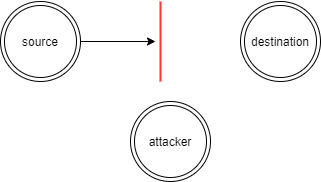
\includegraphics[width=0.37\textwidth]{images/attacks2.png}
	\caption{The attacker interrupts the flow of information}
	\label{fig:attacks2}
\end{wrapfigure}

\begin{definition}
	Interruption: the attacker stops the flow of information (Figure \ref{fig:attacks2}). The attacker interrupts a service, it breaks system integrity and availability.
\end{definition}

\vspace{5mm}
Some examples of interruption:
\begin{example}
	\leavevmode
	%Some examples of interruption:
	\begin{itemize}
		\item the destruction of a part of the hardware
		\item canceling of programs or data files
		\item the destruction of a network link
		\item a denial of service (DoS) that makes the system/network unusable 
	\end{itemize}
\end{example}

\begin{wrapfigure}[6]{l}{0.4\textwidth}
	%\centering
	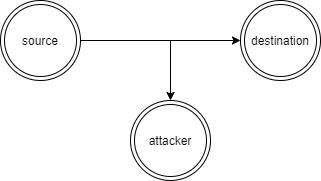
\includegraphics[width=0.37\textwidth]{images/attacks3.png}
	\caption{The attacker intercepts information}
	\label{fig:attacks3}
\end{wrapfigure}

\begin{definition}
	Eavesdropping (interception): the attacker gets unauthorized access to the information (depicted as an additional flow towards the attacker).
\end{definition}

\vspace{5mm}
Interception is an attack to confidentiality, these attacks are hard to detect.
\begin{example}
	\leavevmode
	\begin{itemize}
		\item unauthorized copies of files or programs;
		\item interception of data flowing in the network (a credit card number).
	\end{itemize}
\end{example}
\vspace{15mm}
Interception attacks are hard to detect because source and destination don't notice any change (differently from interruption, where destination don't receive the flow).


\begin{wrapfigure}[6]{l}{0.4\textwidth}
	%\centering
	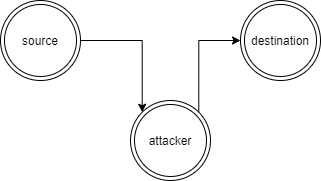
\includegraphics[width=0.37\textwidth]{images/attacks4.png}
	\caption{The attacker modifies information}
	\label{fig:attacks4}
\end{wrapfigure}

\begin{definition}
	Modification: the attacker intercepts the information and make unauthorized modification.
\end{definition}

In this case destination might notice that something is wrong.
\begin{example}
	\leavevmode
	\begin{itemize}
		\item unauthorized change of values (e.g.: of a database);
		\item unauthorized change of a program;
		\item unauthorized change of data flowing in a network;
		\item \texttt{A} redirects \texttt{S}'s bank transfer to herself (either in the browser or in the network, man in the middle).
	\end{itemize}
\end{example}

\begin{wrapfigure}[5]{r}{0.4\textwidth}
	%\centering
	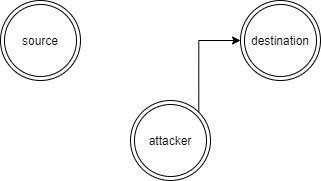
\includegraphics[width=0.37\textwidth]{images/attacks5.png}
	\caption{The attacker forges new information}
	\label{fig:attacks5}
\end{wrapfigure}

\begin{definition}
	Forging (falsification): the attacker inserts new information in the system (usually related to impersonation since the attacker lets the destination believe the information is coming from the honest source). 
\end{definition}

Forging is an attack to \textit{authenticity, accountability} and \textit{integrity}.

\begin{example}
	\leavevmode
	\begin{itemize}
		\item addition of messages in the network;
		\item addition of a record in the database.
	\end{itemize}
\end{example}

\vspace{35mm}

\begin{figure}[H]
	\centering
	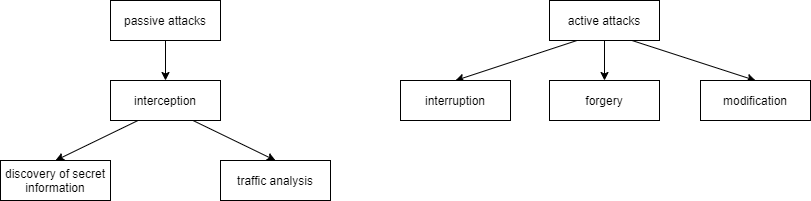
\includegraphics[scale=0.55]{images/typeofattacks.png}
	\caption{Classification of different types of attacks}
	\label{fig:typeofattacks}
\end{figure}
\newpage
\begin{example}
	Suppose a bank B is using the following simple protocol to allow a bank transfer from user Alice (A):\\
	\begin{center}
	\texttt{A $\rightarrow$ B: sign\_A("}please pay Bob 1000€\texttt{")}
	\end{center}
	\texttt{sign\_A} is some "signature" mechanism to ensure that the message really comes from Alice (thus the attacker cannot generate valid signed messages from Alice).
	
	Let's suppose Bob is the attacker, he intercepts the whole message and repeats it as many times as he want, without modifying it. This attack (called replay) consists of an interception plus forging (in this case the message is just re-sent as it is). Bob obtains many bank transfers by just re-sending message M.
\end{example}

\begin{example}
	Program modification: It is an attack to confidentiality, Bob modifies a program that is used by Alice, such a program apparently works normally, however it changes (e.g. the access rules of the users that are executing it, in this case it is called \textit{Trojan horse}). Bob waits that Alice uses the program and copies all the files of Alice in his home directory.
\end{example}

\subsubsection{Cryptography}
The term \textit{cryptography} comes from the greek and means "hidden writing". It is a way to protect the information when the environment is insecure.
For example it is used when the information is sent on a network such as internet or when the system does not support sufficient protection mechanisms.

\begin{definition}
	Encryption: a \textit{plaintext} (message) is transformed using some rules (encryption algorithm) in a ciphertext.
\end{definition}

\begin{definition}
	Decryption: the plaintext is reconstructed starting from a ciphertext.
\end{definition}

The decryption has to be simple for the receiver and unfeasible for an attacker.
The information is encrypted in the source and travels to the destination where it will be decrypted.
In order to do this there are two possible solutions:
\begin{enumerate}
	\item only the sender (Alice) and the receiver (Bob) know the encryption algorithm. If the attacker, by looking at the flow of information, is able to guess which algorithm is used, then he will be able to decrypt all the messages sent;
	\item the encryption algorithm is public and Alice and Bob share some information (the encryption key) non accessible by the attacker. If the attacker doesn't have the encryption key, it is unfeasible to decrypt the messages.
\end{enumerate}

The second solution is better because it is simpler to distribute only one key and if there is an attack it is easier to change key instead of a whole algorithm.

\begin{figure}[H]
	\centering
	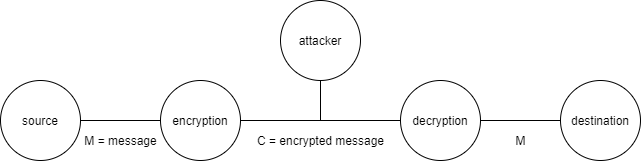
\includegraphics[scale=0.6]{images/enc1.png}
	\caption{Encryption with a shared key}
	\label{fig:enc1}
\end{figure}

We want to build a secure channel to be able to exchange the encryption key.

\begin{figure}[H]
	\centering
	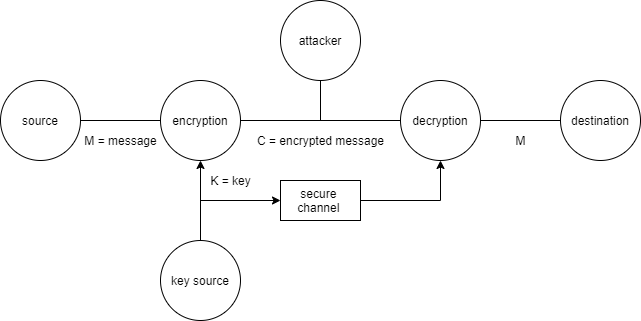
\includegraphics[scale=0.6]{images/enc2.png}
	\caption{Encryption with a shared key and the secure channel}
	\label{fig:enc2}
\end{figure}

This is called \textit{symmetric key cipher} (symmetric because source and destination use the same key).

One of the first encryption algorithms was used by Julius Caesar. In the Caesar Cipher all the letters are permuted using a certain rule (each letter is substituted by the one 3 positions ahead in the alphabet)

\begin{center}
	\texttt{A $\rightarrow$ D\\
	B $\rightarrow$ E\\
	C $\rightarrow$ F\\
	...\\
	Z $\rightarrow$ C}
\end{center}

In this case the algorithm is the Caesar Cipher and the key is 3.

\chapter*{Lecture 2}
The idea behind this course is to build step-by-step a system that is stronger and stronger until we'will arrive to systems that are used in practice.\\

Defining a cipher means to define an encryption algorithm and a decryption algorithm.\\
A \textbf{cryptosystem} (or \textbf{cipher}) can be defined as a quintuple \texttt{(P,C,K,E,D)} where:
\begin{itemize}
	\item \texttt{P} is the set of plaintexts (i.e. all the Italian words);
	\item \texttt{C} is the set of ciphertexts;
	\item \texttt{K} is the set of keys (we can have more than one key);
	\item \texttt{E:K$\times$P$\rightarrow$C} is the encryption function;
	\item \texttt{D:K$\times$C$\rightarrow$P} is the decryption function.
\end{itemize}
Let \texttt{x$\in$P, y$\in$C, k$\in$K}, we will write $E_k$(x) and $D_k$(y) to denote E(k,x) and D(k,y), the encryption and the decryption under the key k of x and y respectively.\\

We require two properties for each cipher that uses a shared key:
\begin{property}
	$D_k(E_k(x)) = x$, decrypting a ciphertext with the right key gives the original plaintext.
\end{property}
\begin{property}
	computing k or x given a ciphertext is infeasible, so complex that cannot be done in a reasonable time.
\end{property}

All the ciphers we will discuss have the first property, only "secure" ciphers have the second one (Caesar cipher doesn't). If someone, one day, will prove that P=NP, then most of the ciphers won't be secure anymore.

\begin{example}
	Referring to the Caesar cipher, we can define the encryption function as "the letter three positions ahead (of our letter x) in the alphabet" or \texttt{(x+3) mod26} and the decryption function as "the letter three position behind (of the letter to be decrypted)" or \texttt{(x-3) mod26}. Our key k=3.
\end{example}

If we find the message \texttt{"BHV BRX PDGH LW"} and we know that it is encrypted with the Caesar cipher we can easily decrypt it into \texttt{"YES YOU MADE IT"} just going back 3 positions. We can notice that we have two "B" and they correspond to the same decrypted letter "Y", in monoalphabetic ciphers this is a strong weakness.

\begin{proof}[Proof of the first property applied to the Caesar cipher]
	We have to prove that:
	\begin{align}
	x &= D_k(E_k(x)) \\
	&=((x+3) \ \textrm{mod}26 - 3) \ \textrm{mod}26 \\
	&=((x+3) - 3) \ \textrm{mod}26 \\
	&=x \ \textrm{mod}26 \\
	&=x
	\end{align}
	Since we have the modules repeated twice we can keep only the external one.
\end{proof}
To prove this property we can apply this reasoning to every cipher.\\

\begin{definition}
	Kerckhoffs' principle: a cipher should remain secure even if the algorithm becomes public.
\end{definition}

Kerckhoffs rules (1883):
\begin{itemize}
	\item The system should be, if not theoretically unbreakable, unbreakable in practice;
	\item The design of a system should not require secrecy, and compromise of the system should not inconvenience the correspondents (Kerckhoffs' principle);
	\item the key should be memorable without notes and should be easily changeable;
	\item the cryptograms should be transmittable by telegraph;
	\item the apparatus or documents should be portable and operable by a single person;
	\item the system should be easy, neither requiring knowledge of a long list of rules nor involving mental strain.
\end{itemize}


The Caesar cipher is clearly insecure (it will be proved later) since once the cipher has been broken any previous exchanged message is also broken (as the cipher works the same way), the key should be changed and it is assumed to be the only secret.

\subsubsection{Shift cipher}
We can extend the Caesar cipher to a shift cipher with a generic key k, we can choose any key in the range $0\leq k\leq 25$. For simplicity we will consider letters as numbers (\texttt{A=0, B=1, .., Z=25}), this means that $P=C=K=Z_{26}$ ($Z_{26}$ is for all the integers between 0 and 25). For the encryption and decryption function we have:
\begin{center}
	$\textrm{E}_k(x) = (x+k) \textrm{mod}26$\\
	$\textrm{D}_k(y) = (y-k) \textrm{mod}26$
\end{center}
The Caesar cipher is a subcase of a shift cipher with k=3.
In  a shift cipher is useless to have k=0 because we would end up with equals plaintexts and ciphertexts.

\begin{example}
	Considering k=10, it gives the following substitution:
	\begin{center}
		\texttt{ABCDEFGHIJKLMNOPQRSTUVWXYZ}\\
		$\downarrow$\\
		\texttt{KLMNOPQRSTUVWXYZABCDEFGHIJ}
	\end{center}
\end{example}

\begin{proof}[Proof of the first property applied to a shift cipher]
	We have to prove that:
	\setcounter{equation}{0}
	\begin{align}
		x &= D_k(E_k(x)) \\
		&=D_k((x+k) \ \textrm{mod}26) \\
		&=((x+k) \ \textrm{mod}26 - k) \ \textrm{mod}26 \\
		&=((x+k) - k) \ \textrm{mod}26 \\
		&=x \ \textrm{mod}26 \\
		&=x
	\end{align}
\end{proof}
Note that $\textrm{Z}_{26}$ is a group under the addition (but not under the multiplication).

\begin{definition}
	A \textbf{group} $\langle\textrm{G},*\rangle$ is a set G together with a (closed) binary operation * on G such that:
	\begin{itemize}
		\item the operator is associative ($(x*y)*z =x*(y*z)$ for all x,y,z in $\langle\textrm{G},*\rangle$);
		\item there is an element e$\in$G such that $a*e = e*a = a$ for all a$\in$G. Such an element is the identity element;
		\item for every a$\in$G, there is an element b$\in$G such that $a*b=e$. This b is said to be the inverse of a with respect to *. The inverse of a is sometimes denoted as $\textrm{a}^{-1}$.
	\end{itemize}
\end{definition}
\vspace{5mm}
The set $\langle\textrm{Z},+\rangle$, which is the set of integers under addition, forms a group:
\begin{itemize}
	\item addition is associative ($(x+y)+z = x+(y+z)$ for all x,y,z in $\langle\textrm{Z},+\rangle$);
	\item the identity element is 0, since $0+a = a+0 = a$ for any a$\in$Z;
	\item the inverse of any a$\in$Z is -a.
\end{itemize}
A group that is commutative with an additive operator is said to be an abelian group.

\vspace{5mm}
The set $\langle\textrm{Z},\cdot\rangle$, the set of all integers under multiplication, does not form a group. There is a multiplicative identity 1 but there is no multiplicative inverse for every element in Z.\\

From now on we will work with abelian groups.

\subsubsection{Possible attack to shift ciphers}
If I can attack a shift cipher, I can implicitly attack the Caesar cipher.
\begin{example}
	If I am an attacker, I see the message \texttt{NGPPS} and I know that it is encrypted using a shift cipher but I don't know which key k is used I can try to get it by trial and error. I start with \texttt{k=1} and if decrypting the message I obtain something nonsense, I try with k=2 and so on. with k=4 I will reach that \texttt{NGPPS=HELLO}. Is it feasible? Yes because we only have 26 possible to keys to try. This type of attack is called \textbf{Brute force}.
\end{example}

In this case the problem with our encryption algorithm is the very small number of keys. Thus the second property doesn't hold (Kerckhoffs' principle: a cipher should remain secure even if the algorithm becomes public). The weakness is that we know that each letter is moved by the same distance.

\subsubsection{Substitution cipher}
A substitution cipher is a generalization to overcome the previous limitation: instead of moving all the letters by the same distance, now we use a generic permutation of the alphabet to map the letters. For example:
\begin{center}
	\texttt{ABCDEFGHIJKLMNOPQRSTUVWXYZ}\\
	$\downarrow$\\
	\texttt{SWNAMLXCVJBUYKPDOQERIFHGZT}
\end{center}
"\texttt{HOME}" becomes "\texttt{CPYM}". In this case the key is the complete permutation, otherwise the receiver is not able to decrypt our message. As for the previous ciphers, to decrypt we just apply the inverse substitution.\\
We have P=C=$\textrm{Z}_{26}$ and K=\{p|p is a permutation of 0,..,25\} with:
\begin{itemize}
	\item $\textrm{E}_k$(x)=$\rho$(x);
	\item $\textrm{D}_k$(y)=$\rho^{-1}$(y).
\end{itemize}

Can we "Brute force" also this type of ciphers? No, we would have to try 26! keys, which is approximately $4\times10^{26}>2^{88}$. This number of keys is very heavy to brute force, even with powerful parallel computers. We have to find something different to attack substitution ciphers. How can we do it?\\

It is a monoalphabetic cipher (it maps a letter to the very same letter), this preserves the statistics of the plaintext and makes it possible to reconstruct the key by observing the statistics in the ciphertext. For example, in Italian, almost all the words end with a vowel, and the vowels (a,e,i,o,u) are easy to identify as they are much more frequent than the other letters.\\

Let us assume a cryptoanalyst knows the used cipher (e.g. a monoalphabetic substitution cipher) and the language used in plaintext (e.g Italian), but he doesn't know the plaintext and the key.

\begin{example}
	Given a ciphertext C, let us compute the frequency of letters, for example lette S appears 0 times and letter C appears 15 times. Is it possible that the cipher transforms A into S, and Z into C (A is never found and Z is found 15 times)? It is possible but very unlikely.
\end{example}

To compute the statistics for letters in Italian language it has been used a text of 14.998 letters, 1/3 from the book "Pinocchio" and 2/3 from the book "Il nome della rosa". The letters frequency are reported in the following table.
\newpage
\begin{table}[h!]
	\centering
	\begin{tabular}{||c | c | c||} 
		\hline
		\textbf{Letter} & \textbf{Absolute frequency} & \textbf{Percentage frequency} \\ 
		\hline\hline
		A & 1714 & 0.114 \\ 
		\hline
		B & 160 & 0.011 \\ 
		\hline
		C & 637 & 0.042 \\ 
		\hline
		D & 566 & 0.038 \\ 
		\hline
		E & 1658 & 0.111 \\ 
		\hline
		F & 141 & 0.009 \\ 
		\hline
		G & 272 & 0.018 \\ 
		\hline
		H & 160 & 0.011 \\ 
		\hline
		I & 1563 & 0.104 \\ 
		\hline
		L & 966 & 0.064 \\ 
		\hline
		M & 436 & 0.029 \\ 
		\hline
		N & 966 & 0.064 \\ 
		\hline
		O & 1486 & 0.099 \\ 
		\hline
		P & 421 & 0.028 \\ 
		\hline
		Q & 85 & 0.006 \\ 
		\hline
		R & 978 & 0.065 \\ 
		\hline
		S & 771 & 0.051 \\ 
		\hline
		T & 1024 & 0.068 \\ 
		\hline
		U & 528 & 0.035 \\ 
		\hline
		V & 343 & 0.023 \\ 
		\hline
		Z & 123 & 0.008 \\ 
		\hline
		\textbf{Total} & \textbf{14998} & \textbf{0.998} \\ 
		\hline
	\end{tabular}
	\label{tab:italianstats}
	\caption{Letters statistics for Italian language.}
\end{table}

The most used letter is A and the less used is Q. We can also build the graph in figure \ref{fig:itastatsgraph} to represent this statistic.
\begin{figure}[H]
	\centering
	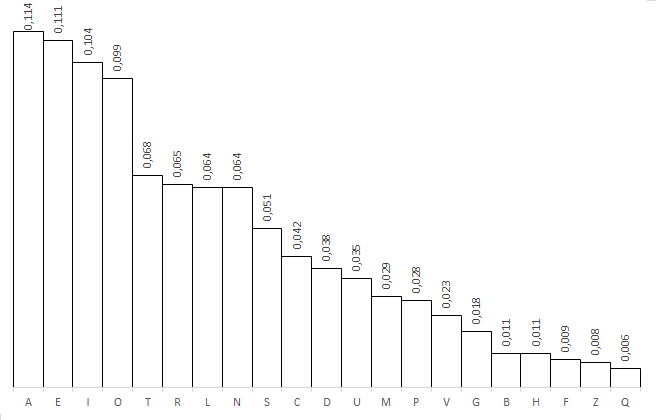
\includegraphics[scale=0.7]{images/Lec2/itastatsgraph.png}
	\caption{Percentage frequencies of letters in Italian language.}
	\label{fig:itastatsgraph}
\end{figure}
Knowing this, we can study the frequency of each letter in my ciphertext and map them using the frequency of my language.
\begin{itemize}
	\item In Italian the frequency of letters I and L increases at the beginning of the sentences (articles "il", "lo", "la"), and the frequency of "A", "E", "I", "O" at the end of the words;
	\item there are words that may appear more frequently (e.g. the word "airplane" in a  military message);
	\item there exist digraph and trigraph that are more frequent. 
\end{itemize}

How can we decrypt a message?
\begin{itemize}
	\item we order the letters of the ciphertext into decreasing frequencies;
	\item we substitute with letters in decreasing order as in the corresponding tables (depending on the language);
	\item there might be mistakes with letters that have the same frequency ("N" and "L" or "H" and "B" in Italian).
\end{itemize}

We need a long ciphertext in order to obtain reasonable frequencies.
It is possible that at the first try we obtain some nonsense words but similar to some words of complete meaning, we can then change letters to correct these words. Repeating some times this step we would end up with the correct plaintext.

We have seen that we can easily break monoalphabetic ciphers applying this method, so the second property doesn't hold. Attacks to substitution ciphers are called \textbf{Statistical attacks}

\begin{proof}[Proof of the first property applied to a substitution cipher]
	We have to prove that:
	\setcounter{equation}{0}
	\begin{align}
		x &= D_k(E_k(x)) \\
		&=D_k(\rho(x)) \\
		&=\rho^{-1}(\rho(x)) \\
		&=x\\
	\end{align}
\end{proof}

We have seen that monoalphabetic ciphers are prone to statistical attacks, since they preserve the statistical structure of the plaintext. A solution are the polyalphabetic ciphers in which the same symbol is not always mapped to the same encrypted symbol.

\subsubsection{Polyalphabetic ciphers}
An example of polyalphabetic cipher is the \textbf{Vigenére cipher} (XVI century). It works on "blocks" of \textit{m} letters with a key of length \textit{m}.
\begin{example}
	The key is \texttt{FLUTE} (m=5). The plaintext is split into blocks of length 5 and the key \texttt{FLUTE} is repeated as necessary and used to encrypt each block.
	\begin{center}
		\texttt{THISISAVERYSECRETMESSAGE}\\
		+\\
		\texttt{FLUTEFLUTEFLUTEFLUTEFLUT}\\
		=\\
		\texttt{YSCLMXLPXVDDYVVJEGXWXLAX}
	\end{center}
	\vspace{5mm}
	Each letter of the ciphertext is given by the sum of the position of the letter in the plaintext plus the position of the letter in the key.
\end{example}
This type of ciphers works better than monoalphabetic ciphers because one letter is not always mapped to the same one unless they are at a distance that is multiple of m.\\

Formally, P=C=K=Z$^m_{26}$, where Z$^m_{26}$ is Z$_{26}\times$Z$_{26}\times$..$\times$Z$_{26}$, m times.
\begin{itemize}
	\item E$_{k1,..,km}$(x$_1$,..,x$_m$) = (x$_1$+k$_1$,..,x$_m$+k$_m$) mod26;
	\item D$_{k1,..,km}$(y$_1$,..,y$_m$) = (x$_1$-k$_1$,..,x$_m$-k$_m$) mod26.
\end{itemize}

If an attacker knows m, he has to try 26$^m$ possible keys, if m is big enough, it is impossible to brute force it.

\chapter*{Lecture 3}

Vigenére cipher cause an almost "flat" distribution of letters frequency, for this reason we would make many mistakes if we try do decrypt a ciphertext in the same way as we do for monoalphabetic ciphers.

As said in the last part of the previous lesson, if we want to brute force this cipher, (assuming we know m) we would have to try 26$^m$ possible keys and that's infeasible, if we don't know m, it would we even worse. It is sufficient to choose m big enough to prevent brute force attacks, note that the number of keys grows exponentially with respect to the length.

\subsubsection{Breaking Vigenére cipher}
Even if the Vigenére cipher hides the statistic structure of the plaintext better than monoalphabetic ciphers, it still preserve most of it.

There are two famous methods to break this cipher, the first is due to Friedrick Kasiski (1863) and the second to Wolfe Friedman (1920). We will see the latter since it is more suitable to be mechanized. Both are based in \textbf{recover the length m of the key} and then \textbf{recover the key}.

The Friedman method uses statistical measures to recover the length m of the key. We consider the index of coincidence:
\setcounter{equation}{0}
\begin{equation}
	I_c(x)=\frac{\sum_{i=1}^{26} f_i(f_i-1)}{n(n-1)} \approx \sum_{i=1}^{26}p_i^2
\end{equation}
where $f_i$ is the frequency of the i-th letter in a text of length n, i.e., the number of times it occurs in such text and $p_i = f_i/n$ is the probability of the i-th letter. Intuitively, this measure gives the probability that two letters, chosen at random from the text, are the same. I compute this probability over all the letters.

\begin{example}
	The IC of \textbf{"the index of coincidence"} is given by:\\
	c(3*2) + d(2*1) + e(4*3) + f(1*0) + h(1*0) + i(3*2) + n(3*2) + o(2*1) + t(1*0) + x(1*0) = \textbf{34}\\
	divided by n(n-1)=21*20 = \textbf{420}\\
	which gives us an IC of 34/420 = \textbf{0.0809}
	
	\vspace{5mm}
	The IC of \textbf{"bmqvszfpjtcsswgwvjlio"} is given by:\\
	b(1*0) + c(1*0) + f(1*0) + g(1*0) + i(1*0) + j(2*1) + l(1*0) + m(1*0) + o(1*0) + p(1*0) + q(1*0) + s(3*2) + t(1*0) + v(2*1) + w(2*1) + z(1*0) = \textbf{12}\\
	divided by n(n-1)=21*20 = \textbf{420}\\
	which gives us an IC of 12/420 = \textbf{0.0286} 
\end{example}

Once I have the IC of my ciphertext, I have to compare it to the ICs of various languages to discover to which it corresponds.

The value of the index is maximum (value 1) for texts composed of just a single letter repeated n times.  The value of the index is minimum (value 1/26 $\approx$ 0.038) for texts composed of letters chosen with uniform probability 1/26.
 
The index of coincidence is thus a measure of how non uniformly letters are distributed in a text, each natural language has a characteristic index of coincidence, some examples:
\begin{center}
	English $\rightarrow$ 0.065\\
	Russian $\rightarrow$ 0.0529\\
	German $\rightarrow$ 0.0762\\
	Spanish $\rightarrow$ 0.0775
\end{center}

We can also use the Friedman method to find moro or polyalphabetic ciphers. We know that if we use frequencies analysis, if frequencies are flat, we have a polyalphabetic cipher, if we have peaks and valleys of frequencies, we have a monoalphabetic cipher. Considering the Friedman method, if the value of the index is minimum $\approx$ 0.038, we have a polyalphabetic cipher, if it is $\approx$ 0.065, we have a monoalphabetic cipher (same IC as English, just a permutation of letters).

With the Friedman method we can estimate m, the length of the key in a Vigenére cipher. The idea is to recover m by brute forcing, following this algorithm (in Python):

\begin{python}
	m=1
	LIMIT = 0.06 #this is to check that ICs are above 0.06 and thus close to 0.065 (assuming the text is in English)
	found = False
	while (not found):
		sub = subciphers() #takes the m subciphertexts sub[m] obtained by selecting one letter every m
		found = True
		for i in range(0,m): #compute the IC of all subtexts
			if IC(sub[i]) < LIMIT:
				#if one of the IC is not as expected try to increase the length
				found = False
				m += 1
				break
	#survived the check, all ICs are above LIMIT
	output (m)
\end{python}
It works because, once we reach the correct m, all the letters we are considering will be encrypted using the same key, "F" in the below example. So, computing the IC, we will obtain a value similar to the English IC value.
\begin{center}
	\texttt{\textcolor{red}{T}HISI\textcolor{red}{S}AVER\textcolor{red}{Y}SECR\textcolor{red}{E}TMES\textcolor{red}{S}AGE}\\
	+\\
	\texttt{\textcolor{red}{F}LUTE\textcolor{red}{F}LUTE\textcolor{red}{F}LUTE\textcolor{red}{F}LUTE\textcolor{red}{F}LUT}\\
	=\\
	\texttt{\textcolor{red}{Y}SCLM\textcolor{red}{X}LPXV\textcolor{red}{D}DYVV\textcolor{red}{J}EGXW\textcolor{red}{X}LAX}
\end{center}

In order to obtain suitable results, we need to have a long enough ciphertext, otherwise we could not be able to succeed.

Now that we have m, we need to find the key. We already said that we cannot brute force it, it would be infeasible. What should we do?
\begin{itemize}
	\item we divide the text into blocks of length m, as the length of the key (we just found it);
	\item we need to build new cryptograms with the first letter of each block, one with the second letter and so on;
	\item we analyse the new cryptograms as before and we find the shift in each position.
\end{itemize}

We are considering texts composed of letter at distance m from the first one, the second one, and so on. They have different shifts, we need to find the relative right shift.

The idea is to shift one subcipher until the mutual index of coincidence with the first subcipher becomes close to the one of the plaintext language, when this happens, we know that the applied shift is the relative shift between the two subciphers and , consequently, between the corresponding letters of the key.

The mutual index of coincidence is defined as:

\setcounter{equation}{0}
\begin{equation}
MI_c(x,x') = \frac{\sum_{i=1}^{26}f_if'_i}{nn'} = \sum_{i=1}^{26} p_ip'_i
\end{equation}
It represents the probability that two letters taken from two texts x and x' are the same.

The following algorithm selects the relative shift that maximizes the mutual index of coincidence.
\begin{python}
	key = [] #empty list
	for i in range(0,m): #for any letter of the key
		k = 0 #current relative shift
		mick = 0 #maximum index so far (we start with 0)
		for j in range(0,26): #for any possible relative shift
			#compute the mutual index of coincidence between the first subcipher
			#sub[0] and the i-th subcipher shifted by j
			mic = MIc(sub[0], shift(j,sub[i]))
			if mic > mick: #if it is the biggest so far
				k = j 		#we remember the relative shift
				mick = mic 	#.. and the maximum
		key.append(k) 		#we append to the list the shift we have found
\end{python}

We repeat this for every letter of the key and we obtain the list of relative shifts, for example, if we obtain [0,4,6,3,9], it means that the second letter of the key is equal to the first plus 4, the third is equal to the first plus 6 and so on. But what is the first letter? The final step is to try all the possible 26 letter of the key, that gives us 26 possible keys.

\subsubsection{Known-plaintext attacks}
Until now we have considered attackers that only know the ciphertext y and try to find either the plaintext x or the key k. It is often the case that an attacker can guess part of the plaintext (e.g., the "standard" header of a message), if a message is split into blocks which are encrypted under the same key, it is reasonable to assume that an attacker can deduce part of the plaintext. For example if the attacker is trying to decrypt an email, he can guess the initial par that often starts with "Dear ...".
If the attacker knows some plaintexts, this gives him the knowledge of some pairs (x,y) plaintext, ciphertext. Given this, the attacker should be able to decrypt other messages or to recover the key k (no matter which cipher is used).

The \textbf{Hill} cipher is a polyalphabetic cipher and it is a generalization of the Vigenére by introducing linear transformations of blocks of plaintext. We have P=C=Z$_m^{26}$, while K=\{K|K is an invertible mod26 matrix m$\times$m\}. The encryption and decryption are the following:
\begin{itemize}
	\item E$_K$(x$_1$,..,x$_m$) = (x$_1$,..,x$_m$)K mod26;
	\item D$_K$(y$_1$,..,y$_m$) = (y$_1$,..,y$_m$)K$^{-1}$ mod26.
\end{itemize}

\begin{example}
	Let us assume M=(x$_1$,x$_2$)=(5,9) and 
		K =$
		\begin{bmatrix}
			5 & 11\\
			8 & 3	
		\end{bmatrix}$
	(we will only consider 2$\times$2 matrices for simplicity). Thus, E$_K$(5,9) = $(5,9)\times
	\begin{bmatrix}
		5 & 11\\
		8 & 3	
	\end{bmatrix}$ mod26 = $(5\times5+9\times8,5\times11+9\times3)$ mod26 = $(25+72,55+27)$ mod26 = $(97,82)$ mod 26 = $(19,4)$
\end{example}

In order to decrypt a message, we need to compute the inverse of the matrix that is our key.
\begin{example}
	We have (y$_1$,y$_2$) = (19,4) and K=$
	\begin{bmatrix}
		5 & 11\\
		8 & 3	
	\end{bmatrix}$. To compute K$^{-1}$:\\
	K$^{-1} = $det$^{-1}$(K) $\begin{bmatrix}
		3 & -11\\
		-8 & 5	
	\end{bmatrix}$ mod26 = det$^{-1}$(K)$
	\begin{bmatrix}
		3 & 15\\
		18 & 5	
	\end{bmatrix}$ mod26.\\
\end{example}

We assume our matrix K is invertible. In the last step we changed the negative numbers to positive ones considering the mod26.

Now we can calculate det(K) = $(5\times3-11\times8)$mod26 = $(15-88)$mod26 = -73 mod26 = 5.
How do we compute det$^{-1}$(K)? To find the inverse mod26 of 5, we need to find a number in the interval [0,25] that multiplied by 5 mod26 gives 1. The number we are searching is 21, $5\times21$ mod26 = 105 mod26 = 1. Thus det$^{-1}$(K) = 21.\\
Note that it is not always the case that the multiplicative inverse modulo exists, we will discuss this more in detail later on, introducing the public key cryptography and RSA.

Now we can solve K$^{-1}$ = det$^{-1}$(K)$
\begin{bmatrix}
	3 & 15\\
	18 & 5	
\end{bmatrix}$ mod26$ = 21
\begin{bmatrix}
	3 & 15\\
	18 & 5	
\end{bmatrix}$ mod26 $=
\begin{bmatrix}
	63 & 315\\
	378 & 105	
\end{bmatrix}$ mod 26 $=
\begin{bmatrix}
	11 & 3\\
	14 & 1	
\end{bmatrix}$. Thus D$_K$(19,4)  = (19,4)$
\begin{bmatrix}
	11 & 3\\
	14 & 1	
\end{bmatrix} = (19\times11+4\times14,19\times3+4\times1)$ mod26 $=(265,61)$ mod26 $=(5,9)$.

\begin{exercise}
	Encrypt and decrypt message (2,5) using a Hill cipher with K = $
	\begin{bmatrix}
		5 & 11\\
		8 & 3	
	\end{bmatrix}$
	
	\vspace{5mm}
	\textbf{Encryption}\\
	E$_K$(2,5) = $(2,5) \times 
	\begin{bmatrix}
		5 & 11\\
		8 & 3	
	\end{bmatrix}$ mod26 $= (2\times5+5\times8,2\times11+5\times3)$ mod26 $=(10+40,22+15)$ mod26 $=(50,37)$ mod26 $=(24,11)$.
	
	\vspace{5mm}
	\textbf{Decryption}\\
	K$^{-1} = $det$^{-1}$(K) $\begin{bmatrix}
		3 & -11\\
		-8 & 5	
	\end{bmatrix}$ mod26 = det$^{-1}$(K)$
	\begin{bmatrix}
		3 & 15\\
		18 & 5	
	\end{bmatrix}$ mod26.\\
	det(K) = $(5\times3-11\times8)$mod26 = $(15-88)$mod26 = -73 mod26 = 5.\\
	det$^{-1}$(K) = 21, $5\times21$ mod26 = 105 mod26 = 1.\\
	K$^{-1}$ = det$^{-1}$(K)$
	\begin{bmatrix}
	3 & 15\\
	18 & 5	
	\end{bmatrix}$ mod26$ = 21
	\begin{bmatrix}
	3 & 15\\
	18 & 5	
	\end{bmatrix}$ mod26 $=
	\begin{bmatrix}
	63 & 315\\
	378 & 105	
	\end{bmatrix}$ mod 26 $=
	\begin{bmatrix}
	11 & 3\\
	14 & 1	
	\end{bmatrix}$.\\
	D$_K$(24,11)  = (24,11)$
	\begin{bmatrix}
	11 & 3\\
	14 & 1	
	\end{bmatrix} = (24\times11+11\times14,24\times3+11\times1)$ mod26 $=(418,83)$ mod26 $=(2,5)$.
\end{exercise}

\chapter*{Lecture 4}

\begin{figure}[H]
	\centering
	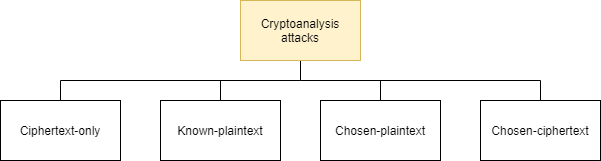
\includegraphics[scale=0.7]{images/Lec4/typesofattacks.png}
	\caption{Types of Cryptonalysis attacks.}
	\label{fig:typesofattacks}
\end{figure}

Up to now we have seen \textbf{ciphertext-only} attacks and \textbf{known-plaintext} attacks (in the last part of the previous lecture).\\
In a ciphertext-only attack, the attacker is assumed to have access only to a set of ciphertexts (e.g., monoalphabetic ciphers, polyalphabetic ciphers), the limit is that it is easy to find the correspondence between letters in the plaintext and in the ciphertext.\\
In a known-plaintext attack, the attacker knows some pairs (x',y'), (x'',y''), .. of plaintexts/ciphertexts (e.g., Hill ciphers), the limit in this case is that it is a linear transformation of plaintext block into a cipher block.

A chosen-plaintext attack (CPA) is an attack model for cryptoanalysis which presumes that the attacker can ask and obtain the ciphertexts for given plaintexts.\\
A chosen-ciphertext attack (CCA) is an attack model for cryptoanalysis where the cryptoanalyst can gather information by obtaining the decryption of chosen ciphertexts.

\begin{exercise}
	Encrypt and decrypt message (1,3) using a Hill cipher with K = $
	\begin{bmatrix}
	1 & 2\\
	4 & 3	
	\end{bmatrix}$
	
	\vspace{5mm}
	\textbf{Encryption}\\
	E$_K$(1,3) = $(1,3) \times 
	\begin{bmatrix}
	1 & 2\\
	4 & 3	
	\end{bmatrix}$ mod26 $= (1\times1+3\times4,1\times2+3\times3)$ mod26 $=(1+12,2+9)$ mod26 $=(13,11)$ mod26 $=(13,11)$.
	
	\vspace{5mm}
	\textbf{Decryption}\\
	K$^{-1} = $det$^{-1}$(K) $\begin{bmatrix}
	3 & -2\\
	-4 & 1	
	\end{bmatrix}$ mod26 = det$^{-1}$(K)$
	\begin{bmatrix}
	3 & 24\\
	22 & 1	
	\end{bmatrix}$ mod26.\\
	det(K) = $(1\times3-2\times4)$mod26 = $(3-8)$mod26 = -5 mod26 = 21.\\
	det$^{-1}$(K) = 5, $21\times5$ mod26 = 105 mod26 = 1.\\
	K$^{-1}$ = det$^{-1}$(K)$
	\begin{bmatrix}
	3 & 24\\
	22 & 1	
	\end{bmatrix}$ mod26$ = 5
	\begin{bmatrix}
	3 & 24\\
	22 & 1	
	\end{bmatrix}$ mod26 $=
	\begin{bmatrix}
	15 & 120\\
	110 & 5	
	\end{bmatrix}$ mod 26 $=
	\begin{bmatrix}
	15 & 16\\
	6 & 5	
	\end{bmatrix}$.\\
	D$_K$(13,11)  = (13,11)$
	\begin{bmatrix}
	15 & 16\\
	6 & 5	
	\end{bmatrix} = (13\times15+11\times6,13\times16+11\times5)$ mod26 $=(261,263)$ mod26 $=(1,3)$.
\end{exercise}

\subsubsection{Attack to the Hill cipher}
If I am an attacker and I have a specific number of pairs (plaintext, ciphertext), I can attack the Hill cipher. With a m$\times$m matrix, I need m pairs, if I have a 2$\times$2 matrix, I will need 2 pairs (plaintext, ciphertext) to be able to extract the key. Once I have the key, I can decrypt all the messages that will be sent later on.

We know that:
\begin{center}
	($y_1^1$, ..., $y_m^1$) = ($x_1^1$, ..., $x_m^1$)K mod26\\
	...\\
	($y_1^m$, ..., $y_m^m$) = ($x_1^m$, ..., $x_m^m$)K mod26\\
\end{center}
which can be written as Y = XK mod26 with:
\begin{center}
	X = $\begin{bmatrix}
		x_1^1 & .. & x_m^1\\
		.. & .. & ..\\
		x_1^m & .. & x_m^m	
	\end{bmatrix}$ and Y = $
	\begin{bmatrix}
		y_1^1 & .. & y_m^1\\
		.. & .. & ..\\
		y_1^m & .. & y_m^m	
	\end{bmatrix}$
\end{center}

If X$^{-1}$ exists, we can write X$^{-1}$Y mod26 = X$^{-1}$XK mod26 and then K = X$^{-1}$Y mod26.

\begin{example}
	Let's define:
	\begin{center}
		x$_1$=(5,9) $\rightarrow$ y$_1$=(19,4)\\
		x$_2$=(2,5) $\rightarrow$ y$_2$=(24,11)
	\end{center}
	We can write (19,4) = (5,9)K mod26 and (24,11) = (2,5)K mod26.\\
	We can construct X and Y matrices as follows:
	\begin{center}
		X = $\begin{bmatrix}
		5 & 9\\
		2 & 5	
		\end{bmatrix}$ and Y = $
		\begin{bmatrix}
		19 & 4\\
		24 & 11	
		\end{bmatrix}$.
	\end{center}
	Now, if X$^{-1}$ exists, we can recover the key K. We compute X$^{-1}$ in the same way we did previously for K$^{-1}$.\\
	X$^{-1}$ = det$^{-1}$(X) $\begin{bmatrix}
		5 & -9\\
		-2 & 5	
	\end{bmatrix}$ mod26 = det$^{-1}$(X) $\begin{bmatrix}
	5 & 17\\
	24 & 5	
	\end{bmatrix}$ mod26.
	
	det(X) = ($5\times5-9\times2$) = (25-18) = 7.\\
	det$^{-1}$(X)  is a number $a$ such that 7$\times a = 1$ mod26, this number $a = 15$.
	
	Thus X$^{-1}$ = det$^{-1}$(X)$\begin{bmatrix}
		5 & 17\\
		24 & 5
	\end{bmatrix}$ mod26 = 15 $\begin{bmatrix}
		5 & 17\\
		24 & 5	
	\end{bmatrix}$ mod26 = $\begin{bmatrix}
	75 & 255\\
	360 & 75	
	\end{bmatrix}$ mod26 = $\begin{bmatrix}
		23 & 21\\
		22 & 23	
	\end{bmatrix}$.
	
	\vspace{5mm}
	Then, K = X$^{-1}$Y mod 26 = $\begin{bmatrix}
		23 & 21\\
		22 & 23	
	\end{bmatrix} \begin{bmatrix}
	19 & 4\\
	24 & 11	
	\end{bmatrix}$ mod26 = $\begin{bmatrix}
		23\times19+21\times24 & 23\times4+21\times11\\
		22\times19+23\times24 & 22\times4+23\times11	
	\end{bmatrix}$ mod26 = $\begin{bmatrix}
		941 & 323\\
		970 & 341	
	\end{bmatrix}$ mod 26 = $\begin{bmatrix}
		5 & 11\\
		8 & 3	
	\end{bmatrix}$.\\
	
	So, our key K = $\begin{bmatrix}
		5 & 11\\
		8 & 3	
	\end{bmatrix}$.
\end{example}

Modern ciphers always contain a non-linear component to prevent this kind of attacks.

If th matrix X is not invertible, if the attacker has no more pairs of (plaintext, ciphertext) he lose, otherwise he can try constructing other X matrices that maybe are invertible.

\subsubsection{Block ciphers}
\textbf{Block ciphers} are cryptosystems that "reuse" the same key to encrypt letters or blocks of the plaintext. For example shift ciphers are part of block ciphers. They are weak because if an attacker know that it is always used the same key, he could recover the key and decrypt al the messages.

\begin{figure}[H]
	\centering
	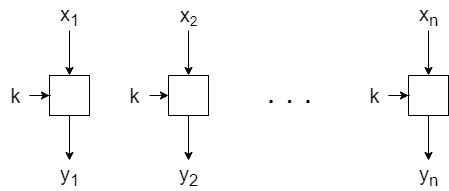
\includegraphics[scale=0.6]{images/Lec4/blockciphers.png}
	\caption{Example of block ciphers.}
	\label{fig:blockciphers}
\end{figure}
\subsubsection{Stream ciphers}
\begin{definition}
	\textbf{Stream ciphers} are cryptosystems that use a stream of key $z_1, z_2, ..., z_n$ instead of a single one.
\end{definition}
The idea is to encrypt the first letter of the plaintext with $z_1$, the second with $z_2$ and so on, it doesn't matter if we encrypt a letter or a block of text, what matters is that the key used is always different.
\begin{figure}[H]
	\centering
	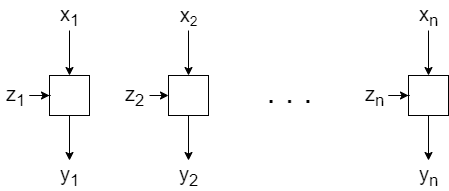
\includegraphics[scale=0.6]{images/Lec4/streamciphers.png}
	\caption{Example of stream ciphers.}
	\label{fig:streamciphers}
\end{figure}

Having a different key for each letter or block of the plaintext is of course appealing but not much practical. The stream of keys is thus usually derived starting from an initial key k, but it can also depend on previous parts of the plaintext. In general we say that
\begin{center}
	z$_i$ = f$_i$(k,x$_i$, ..., x$_{i-1}$).
\end{center}
That means that the i-th key depends on k and on the previous i-1 letters or blocks. So z$_1$ = f$_1$(k), we can compute it without knowledge of the plaintext, to compute z$_2$, instead, we need to know x$_1$ because z$_2$ = f$_2$(k,x$_1$). The values are thus computed in the following sequence: z$_1$, x$_1$, z$_2$, x$_2$, ...\\
This slow down a bit the procedure because I can't do anything in parallel.

Block ciphers are a subset of stream ciphers in which i have z$_i$=k for each i. 

A stream cipher is \textbf{periodic} if its key stream has the form:
\begin{center}
	\texttt{z$_1$, z$_2$, .., z$_d$,z$_1$, z$_2$, .., z$_d$,z$_1$, ...}
\end{center}
So if it repeats after \textbf{d} steps. This form of cipher reminds us to the \textbf{Vigenére cipher}. It can be seen as a stream cipher acting on single letters and with a periodic key stream.

\begin{exercise}
	Formalize the cipher giving (P,C,K,E,D) and defining the key stream z$_i$.
	\begin{itemize}
		\item P=C=K=Z$_{26}$;
		\item E$_{zi}$(x$_i$) = (x$_i$+z$_i$) mod26;
		\item D$_{zi}$(y$_i$) = (y$_i$-z$_i$) mod26;
		\item z$_i$ = k$_{(i \ \text{mod} \ m)}$.
	\end{itemize}
\end{exercise}

A stream cipher is \textbf{synchronous} if its key stream does not depend on the plaintexts (for example z$_i$ = f$_i$(k) for all i). So the key stream can be generated starting from k and independently on the plaintext. It is useful to improve efficiency because we do not need to obtain x$_i$ to compute z$_{i+1}$, so the key stream can be generated offline, before the actual ciphertext is received. We can consider Caesar cipher Hill cipher and also Vigenére cipher part of synchronous ciphers.

\subsubsection{Asynchronous stream ciphers}
In general asynchronous stream ciphers generate keys that depends either from k and from the previous plaintexts:
\begin{center}
	z$_i$ = f$_i$(k, x$_1$, ..., x${i-1}$)
\end{center}
This means that, if we are decrypting, we need to decrypt and, at the same time, compute the keys stream as a key can depend on previous plaintexts. An example is the \textbf{Autokey cipher}. We define it in the same way of a shift cipher, so P=C=K=Z$_{26}$ and
\begin{itemize}
	\item E$_{zi}$(x$_i$) = (x$_i$ + z$_i$) mod26;
	\item D$_{zi}$(y$_i$) = (y$_i$ - z$_i$) mod26.
\end{itemize}
We define the key stream as:
\[ z_i = \begin{cases*}
k & if  i=0  \\
x_{i-1} & if i$\ge$2
\end{cases*} \]%

The first key is the initial key k and the next keys are the same as the previous plaintext.

\begin{figure}[H]
	\centering
	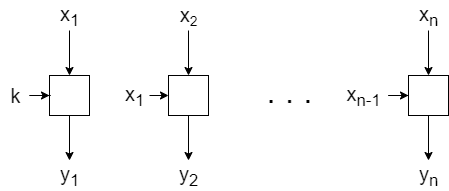
\includegraphics[scale=0.6]{images/Lec4/encautokey.png}
	\caption{Encryption in an autokey cipher.}
	\label{fig:encautokey}
\end{figure}

\begin{exercise}
	Let's assume the plaintext is the word "networksecurity", what is the encryption using k=5?\\
	First of all we need to substitute our word with the corresponding position in the alphabet and it is: "13 4 19 22 14 17 10 18 4 2 20 17 8 19 24". We will encrypt our string as follows:\\
	
	E(13) = (13+5) mod26 = 18\\
	E(4) = (4+13) mod26 = 17\\
	...\\
	E(24) = (24+19) mod26 = 17\\
	
	At this point we just need to transform back our numbers into letters and we obtain the ciphertext.
\end{exercise}

\begin{exercise}
	Try to extract the plaintext from this word encoded using Autokey. We do not know the key k.
	\begin{center}
		\texttt{FTPNIH}
	\end{center}

	Since we do not know the key k, we have to try all the 26 possible k to see which decryption produces a meaningful word.
	
	\begin{itemize}
		\item k=0 will produce \texttt{FOBMWL}, nonsense;
		\item k=1 will produce \texttt{EPANVM}, nonsense;
		\item k=2 will produce \texttt{DQZOUN}, nonsense;
		\item k=3 will produce \texttt{CRYPTO}, it has sense!
	\end{itemize}
\end{exercise}

\begin{exercise}
	Suppose that we know that \texttt{FRIDAY} has been encrypted as \texttt{PQCFKU} using the Hill cipher, What is K? Assume K is a 2$\times$2 matrix.
	
	We can consider the pairs:\\
	\texttt{(F,R) $\rightarrow$ (P,Q) = (5,17) $\rightarrow$ (15,16)}\\
	\texttt{(I,D) $\rightarrow$ (C,F) = (8,3) $\rightarrow$ (2,5)}\\
	\texttt{(A,Y) $\rightarrow$ (K,U) = (0,24) $\rightarrow$ (10,20)}\\
	
	We can construct X and Y matrices as follows:
	\begin{center}
		X = $\begin{bmatrix}
		5 & 17\\
		8 & 3	
		\end{bmatrix}$ and Y = $
		\begin{bmatrix}
		15 & 16\\
		2 & 5	
		\end{bmatrix}$.
	\end{center}
	Now, if X$^{-1}$ exists, we can recover the key K. We compute X$^{-1}$ in the same way we did previously for K$^{-1}$.\\
	X$^{-1}$ = det$^{-1}$(X) $\begin{bmatrix}
	3 & -17\\
	-8 & 5	
	\end{bmatrix}$ mod26 = det$^{-1}$(X) $\begin{bmatrix}
	3 & 9\\
	18 & 5	
	\end{bmatrix}$ mod26.
	
	det(X) = ($5\times3-17\times8$) = (15-136) = -121 mod26 = -17 mod26 = 9.\\
	det$^{-1}$(X)  is a number $a$ such that 9$\times a = 1$ mod26, this number is $a=3$.\\
	
	Thus X$^{-1}$ = det$^{-1}$(X)$\begin{bmatrix}
	3 & 9\\
	18 & 5
	\end{bmatrix}$ mod26 = 3 $\begin{bmatrix}
	3 & 9\\
	18 & 5	
	\end{bmatrix}$ mod26 = $\begin{bmatrix}
	9 & 27\\
	54 & 15	
	\end{bmatrix}$ mod26 = $\begin{bmatrix}
	9 & 1\\
	2 & 15	
	\end{bmatrix}$.
	
	\vspace{5mm}
	Then, K = X$^{-1}$Y mod 26 = $\begin{bmatrix}
	9 & 1\\
	2 & 15	
	\end{bmatrix} \begin{bmatrix}
	15 & 16\\
	2 & 5	
	\end{bmatrix}$ mod26 = $\begin{bmatrix}
	9\times15+1\times2 & 9\times16+1\times5\\
	2\times15+15\times2 & 2\times16+15\times5	
	\end{bmatrix}$ mod26 = $\begin{bmatrix}
	137 & 149 \\
	60 & 107	
	\end{bmatrix}$ mod 26 = $\begin{bmatrix}
	7 & 19\\
	8 & 3	
	\end{bmatrix}$.\\
	
	So, our key K = $\begin{bmatrix}
	7 & 19\\
	8 & 3	
	\end{bmatrix}$.
\end{exercise}

\chapter*{Lecture 5}

\begin{definition}
	A \textbf{perfect cipher} is a cipher that can never be broken, even after an unlimited time.
\end{definition}
But do perfect ciphers exist? Yes, but they are only theoretically (they can be implemented), in practice they are unpractical.

The theory behind perfect ciphers has been developed by \textbf{Claude Shannon}. It assumes an only-ciphertext model of the attacker, this means that the attacker only knows the ciphertext y and tries to find the plaintext x or the key k.

We can provide another definition for perfect ciphers:
\begin{definition}
	A cipher system is said to offer \textbf{perfect secrecy} if, on seeing the ciphertext, the interceptor gets no extra information about the plaintext than he had before the ciphertext was observed. In a cipher system with perfect secrecy, the interceptor is forced to guess the plaintext.
\end{definition}

To formalize them we need to introduce a bit of probability:
\begin{itemize}
	\item p$_p$(x) is the probability of plaintext x to occur;
	\item p$_K$(k) is the probability of certain key k to be used as encryption key.
\end{itemize}
Given a plaintext and a key there exists a unique corresponding ciphertext.

The two probability distributions p$_p$(x) and p$_K$(k) induce a probability distribution on the ciphertexts.
\setcounter{equation}{0}
\begin{equation}
	p_c(y) = \sum_{k \in K, \exists x |E_k(x)=y}^{} p_K(k)\times p_p(D_k(y))
\end{equation}

This means that, given a ciphertext y, we look for all the keys that can give such a ciphertext from some plaintext x. Then we sum the probability of all such keys times the probability of the corresponding plaintext.
\begin{example}
	Let's consider the following toy-cipher with P={a,b}, K={k$_1$,k$_2$}, C{1,2,3}. The encryption is defined in the following table:

	\begin{table}[h!]
		\centering
		\begin{tabular}{|c | c c|} 
			\hline
			\textbf{E} & \textbf{a} & \textbf{b} \\ 
			\hline
			\textbf{k$_1$} & 1 & 2 \\ 
			\textbf{k$_2$} & 2 & 3 \\ 
			\hline
		\end{tabular}
		\label{tab:exmpPerfciph}
	\end{table}

	Let p$_p$(a)=3/4, p$_p$(b)=1/4, p$_K$(k$_1$)=p$_K$(k$_2$)=1/2.
	
	Now we want to compute p$_C$(1), p$_C$(2), p$_C$(3).
	
	p$_C$(1) = p$_p$(a) $\times$ p$_{K}$(k$_1$) = 3/4 $\times$ 1/2 = 3/8\\
	p$_C$(2) = p$_p$(a) $\times$ p$_{K}$(k$_2$) + p$_p$(b) $\times$ p$_{K}$(k$_1$) = 3/4 $\times$ 1/2 + 1/4 $\times$ 1/2 = 3/8 + 1/8 = 1/2\\ 
	p$_C$(3) = p$_p$(b) $\times$ p$_{K}$(k$_2$) = 1/4 $\times$ 1/2 = 1/8\\
\end{example}

\begin{definition}
	The \textbf{conditional probability of a ciphertext} y with respect to a plaintext x, computes how likely is a certain y once we fix x.
	\setcounter{equation}{0}
	\begin{equation}
		p_c(y|x) = \sum_{k\in K, E_K(x)=y}^{} p_K(x)
	\end{equation}
	More simply is just the sum of the probability of all keys giving y from x.
\end{definition}

\begin{example}
	The conditional probability of ciphertext 1 with respect to the two plaintexts a and b is:
	
	\setcounter{equation}{0}
	\begin{align}
		p_c(1|a) &= \sum_{k\in K, E_K(x)=y}^{} p_K(x) = p_K(k_1) = 1/2 \\
		p_c(1|b) &= \sum_{k\in K, E_K(x)=y}^{} p_K(x) = 0		
	\end{align}
	We can notice that 1 can never be obtained from b. Furthermore we can see that if an attacker sees a 1, he can deduce that it is an a, this means that this is not a perfect cipher.
\end{example}

The conditional probability of a plaintext with respect to a ciphertext is related to the security of the cipher. It is a measure of how likely is a plaintext once a ciphertext is observed (which is what the attacker is usually interested to know).

With Pr(y)>0, we can define the \textbf{Bayes' Theorem} as:
\setcounter{equation}{0}
\begin{equation}
	Pr(x|y) = \frac{Pr(x) \times Pr(y|x)}{Pr(y)}
\end{equation}

We can apply this theorem to our case to get the conditional probability of a plaintext x with respect to a ciphertext y:
\setcounter{equation}{0}
\begin{equation}
	p_p(x|y) = \frac{p_p(x) \times p_c(y|x)}{p_c(y)}
\end{equation}

\begin{example}
	At this point we can compute p$_p$(a|1) and p$_p$(b|1) as follows:
	\setcounter{equation}{0}
	\begin{align}
	p_p(a|1) &= \frac{p_p(a) \times p_c(1|a)}{p_c(1)} = \frac{3/4 \times 1/2}{3/8} = 1\\
	p_p(b|1) &= \frac{p_p(b) \times p_c(1|b)}{p_c(1)} = \frac{1/4 \times 0}{3/8} = 0
	\end{align}
\end{example}
Thus, when observing a 1 as a result of a conditional probability of a plaintext x with respect to a ciphertext y, we are sure it is plaintext x, and this means that the cipher is completely insecure.

\begin{exercise}
	What will be the probabilities of plaintexts a and b with respect to ciphertext 3?
	
	First of all we need to find the conditional probabilities of ciphertext 3 with respect to the plaintexts a and b:
	
	\setcounter{equation}{0}
	\begin{align}
		p_c(3|a) &= \sum_{k\in K, E_K(x)=y}^{} p_K(x) = 0 \\
		p_c(3|b) &= \sum_{k\in K, E_K(x)=y}^{} p_K(x) = p_K(k_2) = 1/2		
	\end{align}
	
	We can now compute the conditional probabilities of plaintexts a and b with respect to the ciphertext 3:
	
	\setcounter{equation}{0}
	\begin{align}
		p_p(a|3) &= \frac{p_p(a) \times p_c(3|a)}{p_c(3)} = \frac{3/4 \times 0}{1/8} = 0\\
		p_p(b|3) &= \frac{p_p(b) \times p_c(3|b)}{p_c(3)} = \frac{1/4 \times 1/2}{1/8} =  1
	\end{align}
\end{exercise}

\begin{exercise}
	What if we compute the probabilities of a and b when observing 2?
	
	First of all we need to find the conditional probabilities of ciphertext 2 with respect to the plaintexts a and b:
	
	\setcounter{equation}{0}
	\begin{align}
	p_c(2|a) &= \sum_{k\in K, E_K(x)=y}^{} p_K(x) = p_K(k_1) = 1/2 \\
	p_c(2|b) &= \sum_{k\in K, E_K(x)=y}^{} p_K(x) = p_K(k_2) = 1/2		
	\end{align}
	
	We can now compute the conditional probabilities of plaintexts a and b with respect to the ciphertext 2:
	
	\setcounter{equation}{0}
	\begin{align}
	p_p(a|2) &= \frac{p_p(a) \times p_c(2|a)}{p_c(2)} = \frac{3/4 \times 1/2}{1/2} = 3/4\\
	p_p(b|2) &= \frac{p_p(b) \times p_c(2|b)}{p_c(2)} = \frac{1/4 \times 1/2}{1/2} =  1/4
	\end{align}
\end{exercise}

At this point we can provide an extra definition for perfect ciphers:
\begin{definition}\label{defperfcipher}
	A cipher is perfect iff p$_p$(x|y)=p$_p$(x) for all x in P and for all y in C.
\end{definition}

Intuitively, a cipher is perfect if observing a ciphertext y gives no information about any of the possible plaintexts x.

The cipher in the example is far from being perfect, but it satisfies the above definition for ciphertext 2.

A cipher is perfect if there is some key that maps any message to any ciphertext with equal probability.

\chapter*{Lecture 6}
To prove that a cipher is not perfect, we just need to find a x in P and a y in C that does not satisfy definition \ref{defperfcipher}

\begin{exercise}
	Prove that the shift cipher with p$_K$(k) = 1/|K| = 1/26 (i.e., with keys picked at random for each letter of the plaintext), is a perfect cipher. If we change key at any time we encrypt a letter, the shift cipher becomes perfect (unbreakable).
	
	We can define the cipher as follows:
	\begin{itemize}
		\item P=C=K=Z$_{26}$;
		\item E$_k$(x) = (x+k) mod26;
		\item D$_k$(y) = (y-k) mod26;
		\item k changes at each encryption.
	\end{itemize}
	We want to prove that definition \ref{defperfcipher} holds for this cipher.
	
	We compute the probability of a generic ciphertext y as:
	\setcounter{equation}{0}
	\begin{align}
	p_C(y) &= \sum_{k\in K, \exists x.E_k(x)=y}^{}p_K(k)\times p_p(D_k(y))\\
	&= \frac{1}{26} \sum_{k\in K, \exists x.E_k(x)=y}^{} p_p(D_k(y))\\
	&= \frac{1}{26}\sum_{k\in K}^{}p_p((y-k) mod26)\\
	&= \frac{1}{26}\sum_{x \in P}^{} p_p(x) = \frac{1}{26}
	\end{align}
	
	Note that for each key k, we always have the plaintext (y-k) mod26 that gives y when encrypted under k, and that for all possible keys gives all possible plaintexts x and sums to 1.
	
	\setcounter{equation}{0}
	\begin{align}
	p_c(y|x) &= \sum_{k\in K, E_k(x)=y}^{}p_K(k)\\
	&= p_K((y-x) mod26) =\frac{1}{26}
	\end{align}
	We get that k = (y-x) mod26 from the decryption formula, given x and y, there exists a unique key k that encrypts x as y and it is (y-x)mod26.
	
	Finally we can say that:
	\setcounter{equation}{0}
	\begin{align}
	p_p(x|y) &= \frac{p_p(x)\times p_c(y|x)}{p_c(y)}\\
	&= \frac{p_p(x)\times \frac{1}{26}}{\frac{1}{26}} = p_p(x)
	\end{align}
	We have demonstrated that $p_p(y|x) = p_p(x)$ for all x in P and for all y in C, thus the cipher is perfect.
\end{exercise}

\begin{theorem}\label{theoKP}
	Let $p_c(y)>0$ for all y. A cipher is perfect only if |K|$\ge$|P|.
\end{theorem}

This means that a necessary condition for a cipher to be perfect is that the number of keys is at least the same as the number of plaintexts.
\begin{proof}
	For Bayes' theorem:
		\[p_p(x|y) = \frac{p_p(x)\times p_c(y|x)}{p_c(y)}\]
	Thus, given $p_p(x|y) = p_p(x)$ (the cipher is perfect), we have $p_c(y|x) = p_c(y)$ (these two quantities erase) for all x in P and for all y in C.
	
	As an assumption $p_c(y)>0$.\\
	If we fix x, we obtain that for each y, $p_c(y|x) = p_c(y)>0$. This means that there exists at least one key k such that E$_k$(x)=y (otherwise $p_c(y|x)=0$).
	
	All such keys are different since E$_k$ is a function and we have fixed x, and x cannot be mapped to two different ciphertexts by the same key. Thus, we have at least one key for each ciphertext (|K|$\ge$|C|).
	
	Since, for any cipher (not necessarily perfect), E$_k$ injects the set of plaintexts into the set of ciphertext, we also have |C|$\ge$|P|, thus |K|$\ge$|C|$\ge$|P|, i.e.,
	\begin{center}
		\textbf{|K|$\ge$|P|}
	\end{center}
\end{proof}

\begin{exercise}
	Prove that the ciphertext defined as E$_k$(x$_1$,...,x$_d$)=(x$_1$+k,...,x$_d$+k)mod26 is not perfect.
	
	We can prove this in two ways:
	\begin{enumerate}
		\item using the theorem \ref{theoKP}, proving that |K|<|P|.\\
		Our set K=\{0, 1, 2, .., 25\}, so |K|=26, we need to find |P|. Since x=\{x$_1$,..,x$_d$\} and each x$_i$ can assume 26 values, we have that |P|=26$^d$. Thus 26<26$^d$, so |K|<|P| (with d$\ge$2). 
		\item using definition \ref{defperfcipher}. Let's assume x=\{x$_1$,..,x$_d$\} is an English word and let's also assume d=5. We are looking for an English word of length 5, for example \textit{GOOFY}. Since it is a real word, $p_p$(GOOFY)>0. We want to find a y such that $p_p$(GOOFY|y)$\ne p_p$(GOOFY)>0. For example with y=AAAAA, $p_p$(GOOFY|AAAAA)=0 and we are done. We could have used other y, such as y=ABCDE.
	\end{enumerate}
\end{exercise}

\begin{theorem}\label{theoperfcipher}
	Let |P|=|C|=|K|. A cipher is perfect iff
	\begin{enumerate}
		\item $p_K(k)=1/|K|$ for all k in K;
		\item for each x in P and y in C, there exists exactly one key k such that E$_k$(x)=y.
	\end{enumerate}
\end{theorem}
The theorem states that, for a cipher to be perfect (given that the size of P, C and K is the same), keys should be picked at random for any encryption and each plaintext is mapped into each ciphertext through a unique key.

\begin{proof}
	We will prove the $\rightarrow$ direction of the theorem.
	
	For theorem \ref{theoKP}, in a perfect cipher |K|$\ge$|C| if $p_c$(y)>0 for all y. If we fix x, we obtain that for each y $p_c$(y|x)=$p_c$(y)>0, i.e., there exists at least one key k such that E$_k$(x)=y and all of the other keys are different.
	
	Here (by assumption) |K|=|C|, meaning that all of these keys k are unique (otherwise we would have |K|>|C|). Since this holds for each x and y, we have proved condition 2, i.e., that for each x in P and y in C, there exists exactly one key k such that E$_k$(x)=y.
	
	To prove condition 1, it is enough to notice that given
	\[p_c(y|x) = \sum_{k\in K,E_k(x)=y}^{}p_K(k)\]
	$p_c$(y|x)=$p_p$(y), i.e., the probability of y given x is equal to the probability of the unique key k that encrypts x into y.
	
	Thus, $p_K$(k)=$p_c$(y|x)=$p_c$(y).\\
	If we fix y and we consider all possible plaintexts x we obtain all possible keys k and for all of them it holds $p_K$(k)=$p_c$(y). Since the number of keys is |K|, and since they all have the same probability ($p_c$(y)), and given that the sum of the probabilities of all keys must be 1 and |P|=|C|=|K|, we obtain condition 1, $p_K$(k)=1/|K|.\\
\end{proof}

We can use this theorem to prove that a cipher is (or is not) perfect.
\subsubsection{The one time pad}
This perfect cipher has been used for the telegraph and is a binary variant of Vigenére with keys picked at random.

More precisely we have P=C=K=Z$_{2^d}$ with $p_K$(k)=1/|K|=1/2$^d$ for all k in K. 2$^d$ means sequences of binary numbers of length d.

The encryption function is the following: E$_{k_1,...,k_d}$(x$_1$,...,x$_d$) = (x$_1$ xor k$_1$,...,x$_d$ xor k$_d$), where xor is a bitwise xor operation.

Is it a perfect cipher? Condition 2 of theorem \ref{theoperfcipher} is satisfied by definition. Condition 2 holds too because we are using xor operations.

\subsubsection{Lesson learned}
Shannon theory on perfect ciphers shows that they exist but require as many keys as the possible plaintexts, and keys need to be picked at random for each encryption.

Even if this makes such ciphers unpractical, the one-time-pad has been used for real transmission. The setup consisted of two identical books with thousands of "random" keys. Each key was used only once. Once the book has been used completely, new shared books were necessary.

\chapter*{Lecture 7}
\begin{exercise}
	Consider the following cipher with P=\{a,b\}, K=\{k$_1$,k$_2$,k$_3$\}, C=\{1,2,3,4\}. Encryption is defined by the following table:
		\begin{table}[H]
		\centering
		\begin{tabular}{|c | c c|} 
			\hline
			 & \textbf{a} & \textbf{b} \\ 
			\hline
			\textbf{k$_1$} & 1 & 2 \\ 
			\textbf{k$_2$} & 2 & 3 \\ 
			\textbf{k$_3$} & 3 & 4 \\ 
			\hline
		\end{tabular}
		\label{tab:exerciselec7}
	\end{table}
	We now let $p_p$(a)=1/4, $p_p$(b)=3/4, $p_K$(k$_1$)=1/2, $p_K$(k$_2$) = $p_K$(k$_3$)=1/4.\\
	Compute $p_p$(a|1), $p_p$(a|2), $p_p$(a|3), $p_p$(a|4), $p_p$(b|1), $p_p$(b|2), $p_p$(b|3), $p_p$(b|4).
	
	First of all let's compute all the $p_c$ for 1,2,3,4:
	\[p_c(1) = p_p(a)\times p_K(k_1) = 1/4\times 1/2 = 1/8\]
	\[p_c(2) = p_p(b)\times p_K(k_1)  + p_p(a)\times p_K(k_2)= 3/4\times 1/2 + 1/4\times 1/4 = 7/16\]
	\[p_c(3) = p_p(b)\times p_K(k_2)  + p_p(a)\times p_K(k_3)= 3/4\times 1/4 + 1/4\times 1/4 = 1/4\]
	\[p_c(4) = p_p(b)\times p_K(k_3) = 3/4\times 1/4 = 3/16\]
	
	Then we can compute
	\[p_c(1|a) = p_K(k_1) = 1/2\]
	\[p_c(2|a) = p_K(k_2) = 1/4\]
	\[p_c(3|a) = p_K(k_3) = 1/4\]
	\[p_c(4|a) = 0\]
	
	\[p_c(1|b) = 0\]
	\[p_c(2|b) = p_K(k_1) = 1/2\]
	\[p_c(3|b) = p_K(k_2) = 1/4\]
	\[p_c(4|b) = p_K(k_3) = 1/4\]
	
	Finally:
	\[p_p(a|1) = \frac{p_c(1|a)\times p_p(a)}{p_c(1)} = \frac{1/2\times 1/4}{1/8}= 1\]
	\[p_p(a|2) = \frac{p_c(2|a)\times p_p(a)}{p_c(2)} = \frac{1/4\times 1/4}{7/16}= 1/7\]
	\[p_p(a|3) = \frac{p_c(3|a)\times p_p(a)}{p_c(3)} = \frac{1/4\times 1/4}{1/4}= 1/4\]
	\[p_p(a|4) = \frac{p_c(4|a)\times p_p(a)}{p_c(4)} = \frac{0\times 1/4}{3/16}= 0\]
	
	\[p_p(b|1) = \frac{p_c(1|b)\times p_p(b)}{p_c(1)} = \frac{0\times 3/4}{1/8}= 0\]
	\[p_p(b|2) = \frac{p_c(2|b)\times p_p(b)}{p_c(2)} = \frac{1/2\times 3/4}{7/16}= 6/7\]
	\[p_p(b|3) = \frac{p_c(3|b)\times p_p(b)}{p_c(3)} = \frac{1/4\times 3/4}{1/4}= 3/4\]
	\[p_p(b|4) = \frac{p_c(4|b)\times p_p(b)}{p_c(4)} = \frac{1/4\times 3/4}{3/16}= 1\]
	
\end{exercise}

\subsubsection{Composition of ciphers}
A one-time-pad provides absolute security in theory, but difficult to implement in practice. Modern ciphers are based on very simple operations, such as substitution, xor, etc., that are combined in a smart way so to make the overall algorithm strong and really hard to cryptoanalyse.

Combining simple ciphers does not always improve security. Let's consider the shift cipher composed twice: we first shift by k$_1$ and then by k$_2$ modulo 26. But this is equivalent to shift by k$_1$+k$_2$ modulo 26.

\begin{example}
	Shift of 3 and then of 2:
	\begin{center}
		\texttt{ABCDEFGHIJKLMNOPQRSTUVWXYZ}\\
		\texttt{DEFGHIJKLMNOPQRSTUVWXYZABC}\\
		\texttt{FGHIJKLMNOPQRSTUVWXYZABCDE}\\
	\end{center}
	
	but this is equivalent to a shift of 5:
	\begin{center}
		\texttt{ABCDEFGHIJKLMNOPQRSTUVWXYZ}\\
		\texttt{FGHIJKLMNOPQRSTUVWXYZABCDE}\\
	\end{center}
\end{example}

\begin{definition}
	\textbf{Composition:} we consider two ciphers S$^1$=(P$^1$, C$^1$, K$_1$, E$^1$, D$^1$) and S$^2$=(P$^2$, C$^2$, K$_2$, E$^2$, D$^2$).
	
	We let P$^1$=C$^1$=P$^2$=C$^2$, that we note as P and C in the following. In this way, the output of one cipher is for sure a possible plaintext for the second cipher.
	
	We can now define the composition as S$^1\times$S$^2$=(P, C, K$_1\times$K$_2$, E, D) with:
	\begin{itemize}
		\item E$_{k_1,k_2}$(x) = E$^2_{k_2}$(E$^1_{k_1}$(x));
		\item D$_{k_1,k_2}$(y) = D$^1_{k_1}$(D$^2_{k_2}$(y));
	\end{itemize}
\end{definition}

\begin{exercise}
	Formally apply the composition of the two shift ciphers previously mentioned.
	
	Formally we have E$_k^1$(x)=E$_k^2$(x)=(x+k)mod26\\
	and\\
	E$_{(k_1,k_2)}$(x) = E$_{k_2}^2$(E$_{k_1}^1$(x)) = ((x+k$_1$) mod26+k$_2$) mod26 = (x+(k$_1$+k$_2$)mod26)mod26 = E$_{k_1+k_2mod26}^1$(x)
	
	This proves that composing the shift cipher twice is equivalent to applying it once using as a key the sum of the two keys k$_1$ and k$_2$.
\end{exercise}

\begin{exercise}
	Show that the composition of the shift cipher with the substitution cipher is still a substitution cipher with a different key. Give a constructive way to derive the new key. What happens if substitution is applied before shift? 
	
	Let's consider an example of substitution:
	\begin{center}
		\texttt{ABCDEFGHIJKLMNOPQRSTUVWXYZ}\\
		\texttt{VCFIORBMPLYUQXJHNDWSKETZAG}
	\end{center}
	If we shift of 5 (for example) and then we substitute it becomes:
		\begin{center}
		\texttt{ABCDEFGHIJKLMNOPQRSTUVWXYZ}\\
		\texttt{RBMPLYUQXJHNDWSKETZAGVCFIO}
	\end{center}
	This is nothing more then a substitution cipher with a different key. To decrypt we need to apply first the substitution and then the shift back.
	
	If we do the opposite, so first we substitute and then we shift we would have something similar to the following example:
		\begin{center}
		\texttt{ABCDEFGHIJKLMNOPQRSTUVWXYZ}\\
		\texttt{VCFIORBMPLYUQXJHNDWSKETZAG}\\
		\texttt{AHKNTWGRUQDZVCOMSIBXPJYEFL}
	\end{center}
	Once again it corresponds to a substitution cipher with a different key. Of course to decrypt we would have first to shift back and then substitute.
\end{exercise}

\begin{exercise}
	Consider the composition of a Vigenére cipher with key \texttt{ALICE} with the shift cipher with key 8. Is the resulting cipher equivalent to a known one? If so, what is the resulting key?
	
	The Vigenère cipher with key \texttt{ALICE} encryption can be represented as:
	\begin{center}
		E$_{k_1,...,k_m}$(x$_1$,...,x$_m$) = (x$_1$+0, x$_2$+11, x$_3$+8, x$_4$+2, x$_5$+4, ..) mod26
	\end{center}
	
	A shift cipher with key 8 can be represented as:
	\begin{center}
		\texttt{ABCDEFGHIJKLMNOPQRSTUVWXYZ}\\
		\texttt{IJKLMNOPQRSTUVWXYZABCDEFGH}
	\end{center}

	Then the composition is:
	E$_{k_1,k_2}$(x) = (x$_1$+0+8, x$_2$+11+8, x$_3$+8+8, x$_4$+2+8, x$_5$+4+8, ..) mod26 = (x$_1$+8, x$_2$+19, x$_3$+16, x$_4$+10, x$_5$+12, ..) mod26
	
	This is nothing more then a Vigenére cipher with key \texttt{ITQKM}
\end{exercise}

\subsubsection{Idempotent ciphers}
We have seen that the shift cipher, when repeated twice is equivalent to itself with a different key. When this happens, the cipher is said to be \textbf{idempotent}, written S$\times$S=S. In this case we know that iterating the cipher will be of no use to improve its security, even if we repeat it n times, we will still get the initial cipher, i.e., S$^n$=S.

We have mentioned that modern ciphers are based on simple operations composed together. Almost any modern cipher repeats a basic core of operations for a certain number of rounds (iteration). It is thus necessary that such core operations do not constitute an idempotent cipher.

It can be proved that if we have two idempotent ciphers that commute, i.e., such that S$^1\times$S$^2$=S$^2\times$S$^1$, then their composition is also idempotent. In this case we know that iterating their composition is useless.

\begin{proof}
	Consider one iteration of their composition
	\setcounter{equation}{0}
	\begin{align}
		&(S^1\times S^2)\times(S^1\times S^2)\\
		&=S^1\times (S^2\times S^1)\times S^2 &\text{associative property}\\
		&=S^1\times (S^1\times S^2)\times S^2 &\text{commutative property}\\
		&=(S^1\times S^1)\times (S^2\times S^2) &\text{associative property}\\
		&=S^1\times S^2 &\text{idempotence of the initial ciphers}
	\end{align}
\end{proof} 

\begin{exercise}
	Apply the above result to show that the composition of Vigenére cipher S$^1$ and the shift cipher S$^2$ is idempotent.
	
	The composition is a Vigenére cipher S$^3$ with key k$_1$+k$_2$ mod26, ..., k$_d$+k$_2$ mod26, S$^1\times$S$^2$=S$^3$.
	
	Thus (S$^1\times$S$^2$)$\times$(S$^1\times$S$^2)$ = S$^3\times$S$^3$=S$^3$ which is again a Vigenére cipher with a new key. This holds iterating many times. 
\end{exercise}

We have seen examples of how algebraic properties, such as commutativity, can help simplifying the analysis of a cipher. When developing a robust cipher, we need to avoid as much as possible that operations can be rearranged, swapped, simplified.

\section*{The Advanced Encryption Standard (AES) cipher}
AES has been selected by the National Institute of Standards and Technology (NIST) after a five-year long competition. The original name is Rijndael from the names of the two inventors, Joan Daemen and Vincent Rijmen.

As any modern cipher, AES is the composition of simple operations and contains a non-linear component to avoid known-plaintexts attacks. The composed operation give a non-idempotent cipher that is iterated for a fixed number of rounds.
\newpage
It has been selected since it provides:
\begin{itemize}
	\item high security guarantees;
	\item high performance;
	\item flexibility (different key length)
\end{itemize}
All of these features are, in fact, crucial for any modern cipher.

The Data Encryption Standard (DES) is still in use after almost 40 years, in a variant called Triple DES (3DES), which aims at improving the key length (168 bits). In fact, DES key of only 56 bits(64-8 control bits) is too short to resist brute-forcing on modern, parallel computers.

\subsubsection{Mathematical background of AES}
AES works on the Galois Field with 2$^8$ elements, noted GF(2$^8$). Intuitively it is the set of all 8-bits digits with sum and multiplication performed by interpreting the bits as (binary) coefficients of polynomials. For example 11010011 can be seen as x$^7$+x$^6$+x$^4$+x+1 and 00111010 is x$^5$+x$^4$+x$^3$+x.

The sum of x$^7$+x$^6$+x$^4$+x+1 and x$^5$+x$^4$+x$^3$+x will thus be x$^7$+x$^6$+x$^5$+x$^3$+1 since two 1's coefficient becomes 0 modulo 2=0, and the term disappears. We see that sum and subtraction are just the bit-wise XOR of the binary numbers, 11010011 XOR 00111010 = 11101001 which is x$^7$+x$^6$+x$^5$+x$^3$+1.

The product is done modulo the irreducible polynomial x$^8$+x$^4$+x$^3$+x+1, irreducible means that it cannot be written as the product of two other polynomials, it is, intuitively, the equivalent of primality.
\begin{example}
	(x$^7$+x$^6$+x$^4$+x+1)$\times$ (x$^5$+x$^4$+x$^3$+x) = x$^{12}$ + x$^{11}$ + x$^{10}$ + x$^8$ + x$^{11}$ + x$^{10}$ + x$^9$ + x$^7$ + x$^9$ + x$^8$ + x$^7$ + x$^5$ + x$^6$ + x$^5$ + x$^4$ + x$^2$ + x$^5$ + x$^4$ + x$^3$ + x = x$^{12}$ + x$^6$ + x$^5$ + x$^3$ + x$^2$ + x
	
	Now we need to divide x$^{12}$+x$^6$+x$^5$+x$^3$+x$^2$+x by the irreducible polynomial x$^8$+x$^4$+x$^3$+x+1 and find the reminder. x$^{12}$/x$^8$=x$^4$, thus (x$^8$+x$^4$+x$^3$+x+1)*x$^4$ = x$^{12}$+x$^8$+x$^7$+x$^5$+x$^4$.
	
	At this point we need to subtract this polynomial (to get the remainder), we obtain x$^8$ + x$^7$ + x$^6$ + x$^4$ + x$^3$ + x$^2$ + x and we repeat the process obtain the final remainder: x$^7$ + x$^6$ + x$^2$ + 1.  
\end{example}

\begin{exercise}
	Multiply (x$^4$+x$^3$+1)$\times$(x$^5$+1)
	
	= x$^9$+x$^4$+x$^8$+x$^3$+x$^5$+1 = x$^9$+x$^8$+x$^5$+x$^4$+x$^3$+1
	
	We divide it by the irreducible polynomial: x$^9$/x$^8$ = x, thus (x$^8$+x$^4$+x$^3$+x+1)*x = x$^{9}$+x$^5$+x$^4$+x$^2$+x.
	
	We subtract this polynomial from the result of the multiplication to obtain the reminder: x$^8$+x$^3$+x$^2$+x+1.
	
	We repeat the process and we obtain the final reminder x$^4$+x$^2$.
\end{exercise}
\end{document}


